\documentclass{scrartcl}
\usepackage[utf8]{inputenc}
\usepackage[english]{babel} % Trennung nach der neuen deutschen Rechtschreibung
\usepackage[utf8]{inputenc}
\usepackage[T1]{fontenc}
\usepackage{lmodern}
\usepackage{subcaption}
\usepackage{chemformula}
\usepackage{placeins}
\usepackage{multirow}
\usepackage{enumitem}
\usepackage{amssymb}
\usepackage{amsmath} % Erweiterte Mathematik-Umgebung
\usepackage{amsfonts} % zusätzliche Mathematik-Schrifttypen (v.a. \mathbb für Mengen)
\usepackage{ulem}
\usepackage{amsthm}
\usepackage{graphics}%soll beim Graphiken einfügen hilfreich sein
\usepackage{graphicx}
\usepackage{wrapfig}%lässt Textumflossene Bildeinbindung zu
\usepackage{epstopdf}%soll eps in pdf umwandeln
\usepackage{placeins}
\usepackage{amsthm}
\usepackage{subcaption}
\usepackage{wrapfig}
\usepackage{float}
\usepackage{hyperref}
\usepackage{ragged2e}

\usepackage[a4paper, portrait, margin=2.5cm]{geometry}

\setlength\parindent{0pt}

\begin{document}

\begin{titlepage}
    \begin{center}
        \vspace*{1cm}
        \Huge
        \textbf{Laser}
        
        \vspace{0.5cm}
        \LARGE
        Advanced Lab Course
        
        \vspace{1.5cm}
        \textbf{Louis-Hendrik Barboutie (020157041C), Frederik Ehl (0201719742) and Florence Schmerber (0201845640)}
        
        \vspace{1cm}
        Jörg Baller
        \vfill
        

        \includegraphics[width=0.4\textwidth]{logo_uni.jpg}
        
        \Large
        $05^{\underline{\text{th}}}$ May 2022
    \end{center}
\end{titlepage}

\section{Introduction}

Since their invention in the 1950's, LASER's have found widespread applications in communication, medicine, research and weaponry. The acronym stands for \textit{Light Amplification by Stimulated Emission of Radiation} \cite{laser}. As the acronym suggests, a laser emits light when pumping energy into a light-emitting active medium, eg. ruby or a gas. The atoms in the material are put in excited states, and they release the excess energy as light. When this light is focused into the material again via an optical resonator, it gives rise to induced emissions, whose intensity are much greater than from spontaneous emissions.

This lab class will focus on the study of a gas discharge laser, as depicted in fig.~\ref{fig:gasDischargeLaser}. 
\begin{figure}[!ht]
    \centering
    \includegraphics[width=0.8\textwidth]{IntroBilder/gasDischargeLaser.png}
    \caption{Schematic of a He+Ne gas discharge laser}
    \label{fig:gasDischargeLaser}
\end{figure}

\section{Theory}
A laser consists of three principal components, an active medium, in this case a helium-neon gas, an energy pump and an optical resonator. 
\begin{figure}[H]
    \centering
    \includegraphics[width=0.8\textwidth]{IntroBilder/laserSchematic.png}
    \caption{Schematic of a laser}
    \label{fig:my_label}
\end{figure}
The energy pump, an electric field build up between  an  anode  and  a  cathode, energizes mostly the helium atoms from the ground state into an excited state. The excited helium atoms collide with neon atoms, exciting them in the process. Without helium, the neon atoms would be excited mostly to lower excited states, for which lasing can not be achieved. 
An atom in an excited state is subject to spontaneous emission, where it decays into a lower energy state and a photon with a frequency corresponding to the energy difference between the two levels is emitted. 
\[E_2-E_1=\Delta E= hf_{12}\]
If an already excited atom is hit by a photon, with a frequency corresponding to the energy gap $\Delta E$ of the excited state to ground state transition, the atom falls into the ground state, thereby releasing a second coherent photon of the same frequency and phase. This phenomenon is called stimulated or induced emission and is one of the fundamental processes that led to the development of the laser. Both spontaneous and stimulated emission are stochastical phenomena, described by the Einstein coefficients $A_{21}$ and $B_{21}$ respectively. The rate at which the atoms decay is thereby proportional to the the population $N_2$ of the excited state, i.e. the number of atoms in that state. The incoherent photons are fed back into the active medium by the optical resonator. Some of these photons are being absorbed by atoms in the ground state, while others cause stimulated emission in excited atoms, producing further coherent photons. Optical amplification takes place. In order to produce an efficient laser, the rate of stimulated emission must be higher, than the rate of absorption. Therefore the population of excited-state atoms $N_2$ has to be greater, than the population of ground-state atoms $N_1$.
For a group of atoms at thermal equilibrium, the ratio of the number of atoms in each state is given by the ratio of two Boltzmann distributions:
\[\frac{N_2}{N_1}=e^{\frac{-(E_2-E_1)}{kT}}\]
However, for a system at thermal equilibrium, $N_2$ can never exceed $N_1$, therefore in order to achieve population inversion, the system needs be pushed into a non-equilibrated state.\\


\begin{wrapfigure}{r}{0.4\textwidth}
    \centering
    \includegraphics[width=0.35\textwidth]{IntroBilder/populationInversion.png}
    \caption{Graph representing population inversion}
    \label{fig:popInv}
\end{wrapfigure}
Most common lasers today are 4-level laser, meaning that 4 energy levels are involved, in order to achieve the lasing condition. The pumping transition excites the atoms from the ground state (level 1) into the pump band (level 4). The transitions $4\longrightarrow3$ and $2\longrightarrow1$ occur fast and non-radiative, while the lifetime of the laser transition ($3\longrightarrow2$) is much longer, which results in an accumulation of atoms in level 3, the upper-laser level. Due to the fast transition from level 2 into the ground state, the population of level 2 will essentially be zero, and a population inversion of level 3 with respect to level 2 has been achieved. Optical amplification can now take place at the frequency $f_{32}$. In our case the upper-laser level is the Ne(5s) state, which decays to Ne(3p) by emitting red light (632.8 nm).

The remaining step in utilizing optical amplification to create an operable laser is to place highly reflecting mirrors at each end of the active medium, so that a wave will reflect back upon itself, gaining more power in each pass than is lost due to transmission through the mirrors and diffraction. \cite{HeNeLaser}\cite{popInv}\cite{Einstein}
\section{Method}

\subsection{Lasing condition}
In order to obtain a laser, the mirrors in the resonator need to be aligned with high accuracy, so that light amplification occurs. We have control over three translational axes and three rotational axes, to change position and rotation of the mirror.
First we close the diaphragm to ensure that there is no laser. Then by changing the vertical and horizontal position of the mirror we try to center the light of the gas discharge on the mirror, as well as the back-reflection onto the diaphragm. When done correctly, the lasing condition is fulfilled and a red laser appears even with the closed diaphragm.
To further improve the alignment, we bring a sensitive power meter into the laser beam. The diaphragm is opened and by slightly modifying the orientation of the mirror, we try to maximize the power of the laser beam, by monitoring the reading on the power meter.

\subsection{Polarization}
In a next step we study the polarization of the laser by installing a adjustable polarizer into the laser beam in front of the power meter. We change the orientation of the polarizer in steps of $15^{\circ}$ and monitor the change in power.

\subsection{Study of stability conditions of the cavity}
Next the power of the laser as a function of the length of the resonator is studied. Therefore the distance between the two mirrors is varied by moving the second mirror in steps of 1 cm. Due to the high sensitivity of the instrument, the mirror orientation needs be optimized again after each variation of it's position. It might even occur that the alignment of the mirrors gets lost while changing the position, at which point the lasing condition needs to be restored and re-optimized. 

\subsection{Transversal modes}
Using a camera we record several images of the laser structure, when applying different mirror orientations in order to produce different transversal modes. The polarizer needs to be installed in front of the camera to reduce the intensity of the incoming light, as the image would be too saturated without any polarization.

\subsection{Study of the beam divergence}
In this part of the experiment several images of the same transversal mode are recorded at different distances from the resonator. Using the program ImageJ, the individual diameters of the laser beam on each image is measured and compared.

\section{Results and discussion}


\subsection{Polarization}
After properly adjusting the laser we can study the effect of a polarizer applied on a laser beam.

\begin{figure}[!ht]
\centering
\parbox{0.4\textwidth}{
\begin{footnotesize}
    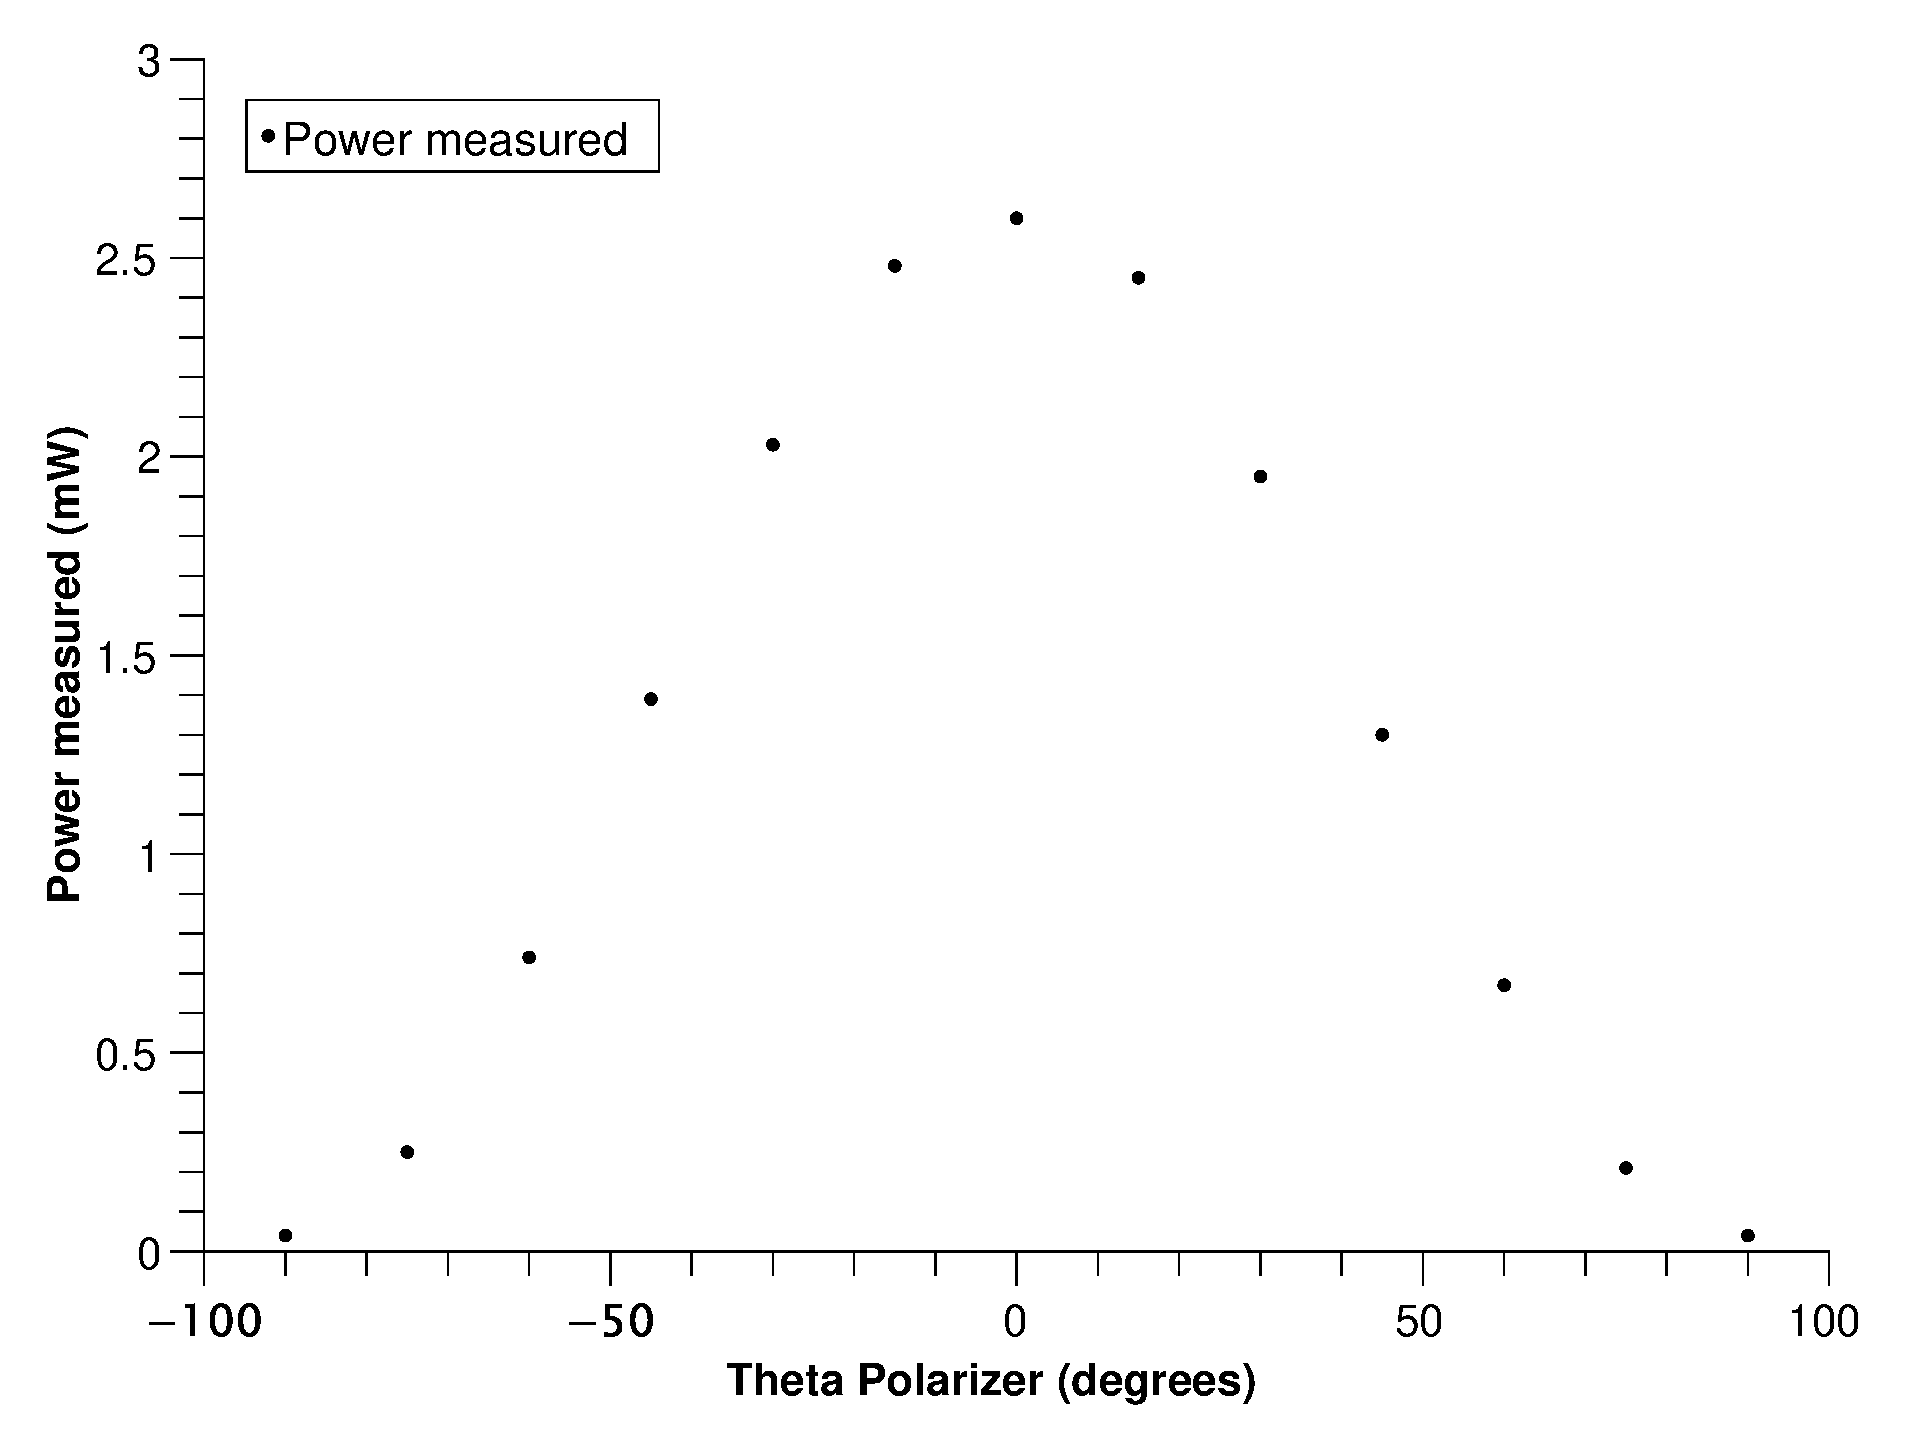
\includegraphics[width=0.47\textwidth]{Polarization.eps}
\end{footnotesize}
}
\qquad
\begin{minipage}[c]{0.53\textwidth}%
\centering
    \begin{tabular}{c|c}
    Angle of polarizer ($^\circ$) &  Power (mW)\\
    \hline
    90 & 0.04 \\
    75 & 0.21 \\
    60 & 0.67 \\
    45 & 1.30 \\
    30 & 1.95 \\
    15 & 2.45 \\
    0 & 2.60 \\
    -15 & 2.48 \\
    -30 & 2.03 \\
    -45 & 1.39  \\
    -60 & 0.74 \\
    -75 & 0.25 \\
    -90 & 0.04
    \end{tabular}
\end{minipage}
\caption{Power as a function of the angle of the polarizer}
\label{fig:polarizer}
\end{figure}
\FloatBarrier

Note that this pattern is periodic, with period of 360°. Only a range of 200° containing the maximum of measured power is represented in fig.~\ref{fig:polarizer}. It is attained for a rotation of 0° of the polarizer. With every change of the orientation of the polarizer, the measured power diminishes. This implies that the light emitted from the laser is itself polarized. When the power measured is maximum, the polarizations of the light from the laser and the polarizer are the same.


\subsection{Cavity stability}

\begin{figure}[!ht]
\centering
\parbox{0.4\textwidth}{
\begin{footnotesize}
    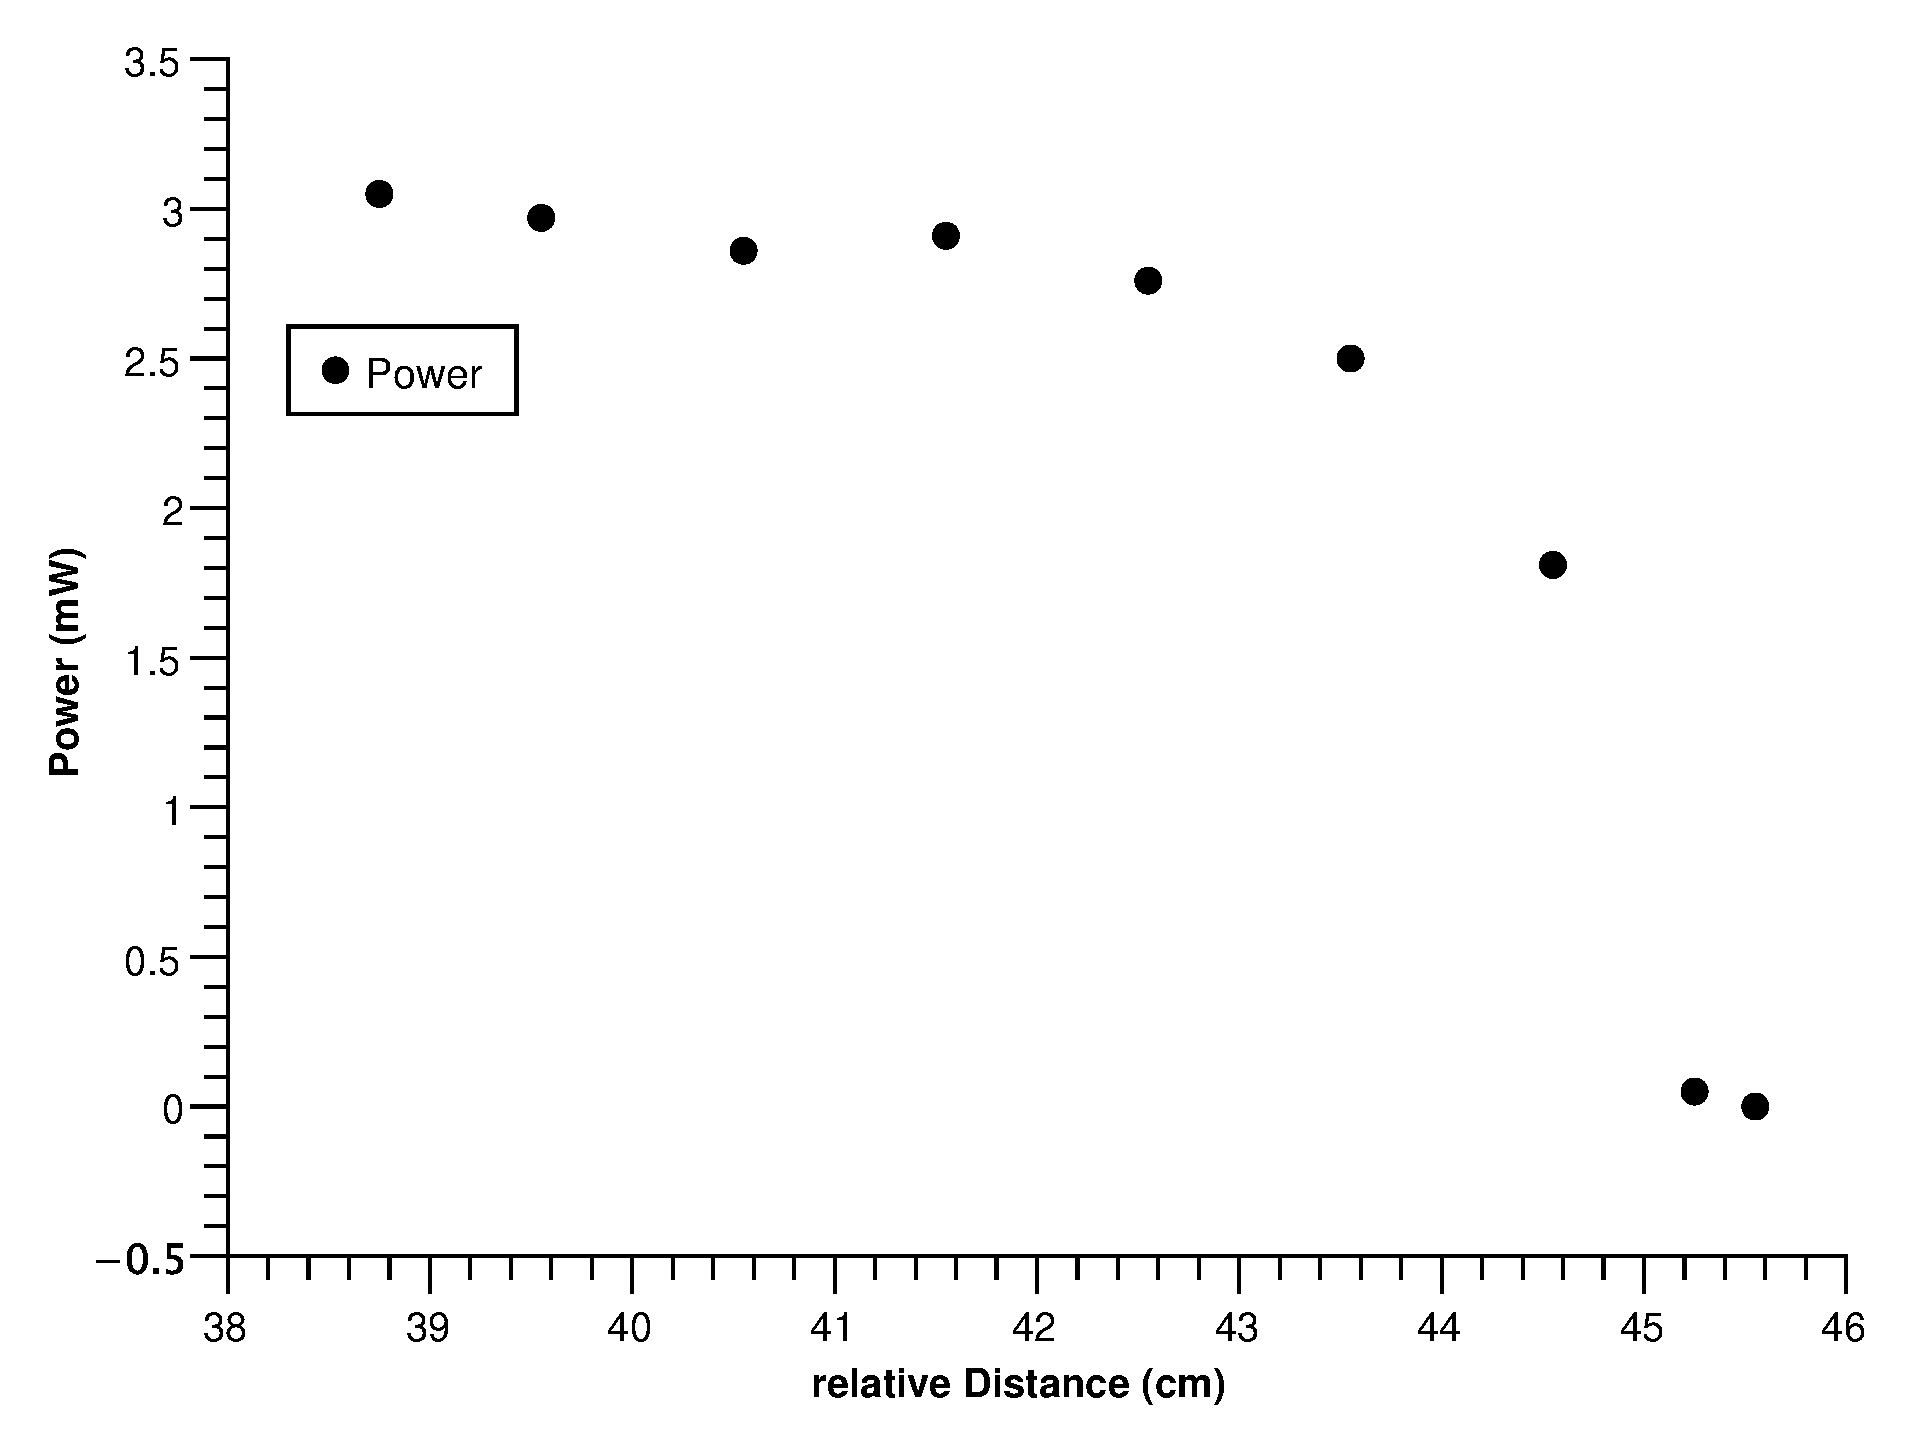
\includegraphics[width=0.47\textwidth]{distance.eps}
\end{footnotesize}}
\qquad
\begin{minipage}[c]{0.53\textwidth}%
\centering
    \begin{tabular}{c|c}
        Distance (cm) & Power (mW) \\
        \hline
        38.75 & 3.05 \\
        39.55 & 2.97 \\
        40.55 & 2.86  \\
        41.55 & 2.91 \\
        42.55 & 2.76 \\
        43.55 & 2.50 \\
        44.55 & 1.81 \\
        45.25 & 0.05 \\
        45.55 & 0.00
    \end{tabular}
\end{minipage}
\caption{Power of the laser as a function of the distance}
\end{figure}
\FloatBarrier

The power drop is first linear and minimal. At about 42 cm, a sharper drop-off is noticeable. After this point the power drops very quickly, and obtaining a laser is not possible anymore.

\subsection{Transversal modes}
Using the camera, and modifying the orientation of the mirror, we obtain images of the transverse modes. We had difficulties obtaining basic transverse modes, but obtained nice pictures of complex transverse mode patterns, as seen in fig.~\ref{fig:transversalModes}.

\begin{figure}[!htb]
    \centering
    \begin{subfigure}{0.45\textwidth}
      \centering
      \includegraphics[width = 1.2 \textwidth]{BilderFleck/2.png}
      \caption{some mode}
      \label{fig:modeA}
    \end{subfigure}
    \hfill
    \begin{subfigure}{0.45\textwidth}
      \centering
      \includegraphics[width = 1.2 \textwidth]{BilderFleck/bilder.png}
      \caption{some other mode}
      \label{fig:modeB}
    \end{subfigure}
    \caption{Transversal modes}
    \label{fig:transversalModes}
\end{figure}
\FloatBarrier

\newpage
\subsection{Study of the beam divergence}
\begin{table}[!ht]
    \centering
    \begin{tabular}{c|c|c}
        Distance (cm) & Total Diameter (pixels) &  Diameter peak-peak (pixels)\\
        \hline
         70 & 460 & 226 \\
         75 & 470 & 237 \\
         80 & 452 & 240 \\
         85 & 466 & 255\\
         90 & 475 & 241 \\
         95 & 483 & 264 \\
         100 & 497 & 247 \\
         105 & 504 & 267 \\
         110 & 514 & 275 \\
         115 & 521 & 284
    \end{tabular}
    \caption{Measured diameter of the laser with corresponding distance of the camera with respect to the resonator}
    \label{tab:beamDiv}
\end{table}
\FloatBarrier

The peak-peak diameter data yields the following graph:
\begin{figure}[H]
    \centering
    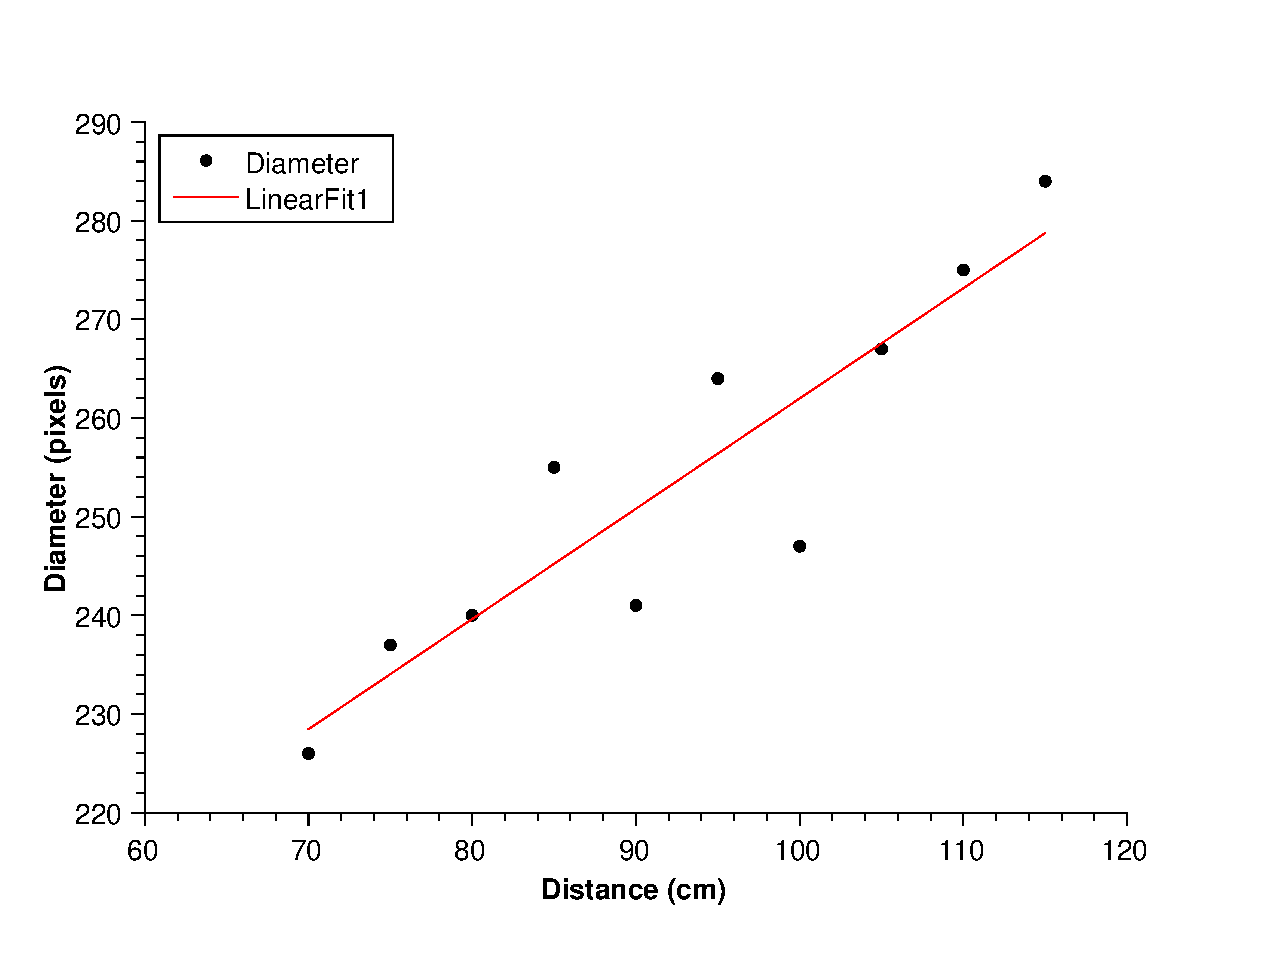
\includegraphics[width=0.6\textwidth]{beam_div.eps}
    \caption{The diameter of the laser as a function of the distance of the camera}
    \label{fig:beam_div}
\end{figure}
We apply a linear fit, whose slope $s$ is given by:
\[s = (1.11 \pm 0.17) \ \text{pixel $\cdot$ cm}^{-1}\] 

As seen on figure \ref{fig:beam_div}, the diameter of the laser becomes larger the further away we observe it. While very focused, the beam still diverges, which means that not all light beams exit the laser in parallel, but with a slight angle. The magnitude of divergence may be reduced by increasing the accuracy in the orientation of the mirrors of the resonator.

\newpage
\subsection{Spectral analysis}

\begin{figure}[!ht]
    \centering
    \begin{subfigure}[b]{0.49\textwidth}
      \centering
      \resizebox{0.8\textwidth}{!}{\includegraphics[width = 1.2 \textwidth]{lichtSpektra/NeonLamp.pdf}}
      \caption{Spectrum of a neon gas discharge lamp}
      \label{fig:neonLamp}
    \end{subfigure}
    \hfill
    \begin{subfigure}[b]{0.49\textwidth}
      \centering
      \resizebox{0.8\textwidth}{!}{\includegraphics[width = 1.2 \textwidth]{lichtSpektra/helium.pdf}}
      \caption{Spectrum of a helium gas discharge lamp}
      \label{fig:heliumLamp}
    \end{subfigure}
    \caption{Spectra of gas discharge lamps}
    \label{fig:lampSpectra}
\end{figure}
\FloatBarrier

\begin{figure}[!ht]
    \centering
    \begin{subfigure}{0.49\textwidth}
      \centering
      \resizebox{0.8\textwidth}{!}{\includegraphics[width = 1.2 \textwidth]{lichtSpektra/NoLaser.pdf}}
      \caption{Spectrum of the light with no laser}
      \label{fig:noLaser}
    \end{subfigure}
    \hfill
    \begin{subfigure}{0.49\textwidth}
      \centering
      \resizebox{0.8\textwidth}{!}{\includegraphics[width = 1.2 \textwidth]{lichtSpektra/Laser.pdf}}
      \caption{Spectrum of the light with the laser}
      \label{fig:yesLaser}
    \end{subfigure}
    \caption{Spectra of the light emitted by the laser, with and without fulfilling the lasing condition}
    \label{fig:laserSpectra}
\end{figure}
\FloatBarrier

We observe that the spectrum of the light without the laser has the same peaks as for the helium and neon lamps. There is a lot of "noise" and not many peaks are clearly defined as for helium. This is due to the many possible energy transitions of neon, each transition releasing light at a unique wavelength. Once we reach the lasing condition however, only one peak appears on the spectrum at around 632 nm. This peak is characteristic for the Ne(5s)->Ne(3p) transition, which is the one emitting the strongest light.

\section{Conclusion}
During this experiment, we familiarized ourselves with the functionality of a laser and studied many different properties such as the stability, transversal modes, beam divergence and the polarization. Moreover, we studied the emission spectra of the laser compared to the helium and  neon gas discharge lamp and the one of the laser tube without lasing, where we verified, that the light of a laser consists of a single wavelength with a single polarization. Unfortunately the experiment is limited to qualitative observations, but lacks some quantitative analysis. For example it would have been nice to determine the beam divergence angle, or go deeper in the study of the transversal modes.
%we learned ...
%(cavity stability) The length of the cavity/mirrors shouldn't be too big, since at some point it not possible anymore to obtain a laser if the second mirror is too far away, meaning that the laser resonator isn't stable.

\begin{thebibliography}{}
    \bibitem{labguide} \textit{Laser}, Advanced lab course guide, Jörg Baller, 2022  
    \bibitem{laser} \textit{Laser}, Wikipedia, \url{https://en.wikipedia.org/wiki/Laser}, last accessed 18/05/2022
    \bibitem{popInv} \textit{Population inversion}, Wikipedia, \url{https://en.wikipedia.org/wiki/Population_inversion}, last accessed 21/05/2022
    \bibitem{HeNeLaser} \textit{Helium-neon laser}, Wikipedia, \url{https://en.wikipedia.org/wiki/Helium-neon_laser}, last accessed 28/05/2022
    \bibitem{Einstein} \textit{Einstein coefficients}, Wikipedia, \url{https://en.wikipedia.org/wiki/Einstein_coefficients}, last accessed 28/05/2022
    
\end{thebibliography}

\end{document}
